\documentclass[conference]{IEEEtran}
\IEEEoverridecommandlockouts
% The preceding line is only needed to identify funding in the first footnote. If that is unneeded, please comment it out.
\usepackage{cite}
\usepackage[spanish]{babel}
\usepackage{listings}
\usepackage{amsmath,amssymb,amsfonts}
\usepackage{algorithmic}
\usepackage{graphicx}
\usepackage{textcomp}
\usepackage{xcolor}
\def\BibTeX{{\rm B\kern-.05em{\sc i\kern-.025em b}\kern-.08em
    T\kern-.1667em\lower.7ex\hbox{E}\kern-.125emX}}
\graphicspath{ {images/} }
\renewcommand{\spanishtablename}{Tabla}%renombrar tablas en español%
\begin{document}

\title{Practica 1 \\ Predicción de rendimiento de gasolina en millas por galón de un auto mediante técnicas de regresión}

\author{\IEEEauthorblockN{1\textsuperscript{st} Erick Franco Gaona}
\IEEEauthorblockA{\textit{Departamento de Estudios Multidisciplinarios} \\
\textit{Universidad de Guanajuato}\\
Yuriria, México \\
e.francogaona@ugto.mx}
}

\maketitle

\begin{abstract}
Las regresiones se utilizan a menudo para predecir situaciones de la vida real en la industria y la ciencia. Existen diversas técnicas para realizar regresiones como pueden ser regresiones lineales multiples o bosques aleatorios. En este trabajo se presenta un caso de estudio de esas dos técnicas sobre un conjunto de datos público para revisar la diferencia de efectividad entre ambos métodos. Mientras que la regresión lineal multiple obtuvo un 82\% de efectividad, los bosques aleatorios obtuvieron un 88\% a costa de un mayor tiempo de ejecución.  
\end{abstract}

\section{Introducción}

El análisis de regresión se usa ampliamente para hacer predicciones y estimaciones de expectativas condicionales de variables dependientes e independientes, y sus aplicaciones se superponen con el campo del aprendizaje automático. Ejecutar regresiones permite determinar los factores más importantes, los factores que a menudo se pasan por alto y cómo se influyen entre sí. Estos factores se denominan variables y se clasifican de la siguiente manera: \\

\begin{itemize}
\item Variable dependiente: Es el factor el cual se está tratando de entender o predecir (Y).
\item Variable(s) independiente(s): Es el factor que se cree que puede impactar en la variable dependiente (X). \\
\end{itemize}

Debido a eso la regresión suele usarse en las organizaciones ya que puede interpretar fenómenos y hacer predicciones sobre el futuro, así como obtener información empresarial valiosa y procesable. Este método proporciona información sobre cómo la estructura de costos y las características variables afectan el producto. Realizar análisis de regresión permite tomar decisiones comerciales más informadas y eficientes y desarrollar estrategias para mejorar la calidad de sus productos y servicios, lo que beneficia a su organización.

La Figura 1 muestra cómo se relaciona el salario con los años de experiencia, prediciendo el salario de un trabajador dado. La regresión muestra una relación lineal positiva entre el salario (eje y) y los años de experiencia (eje x). Puede utilizar estos datos históricos para realizar previsiones salariales. En este trabajo se presentan dos metodos para realizar regresiones y se compara la efectividad de ambos aplicados para la predicción del rendimiento de la gasolina en millas por galón tomando un conjunto de datos público (mpg-auto) de diversos autos.

\begin{figure}[h]
    \centering
    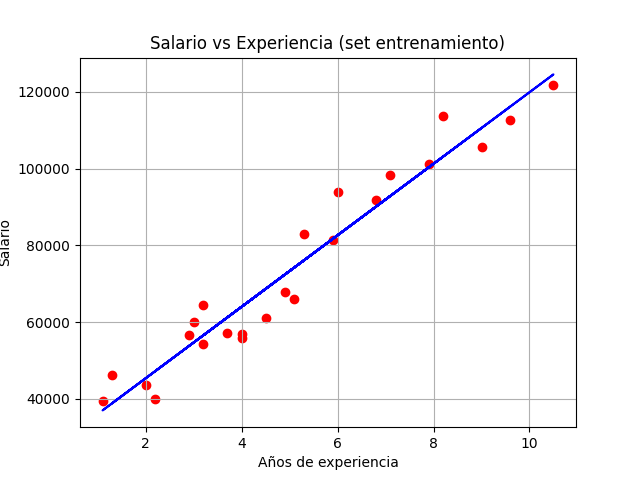
\includegraphics[scale=0.6]{1.png}
    \caption{Ejemplo de regresión aplicado en el salario vs los años de experiencia.}
    \label{fig:mesh1}
\end{figure}

\section{Teoría}
\subsection{Regresión lineal simple}
El análisis de regresión lineal simple se utiliza para predecir el valor de una variable en función del valor de otra variable. La regresión lineal se ajusta a una línea recta o a una superficie que minimiza las diferencias entre los valores de salida y los reales \cite{b1}. Una forma razonable de relación entre la respuesta Y y el regresor x es la relación lineal

\begin{equation}
Y= \beta_0 + \beta_1x
\end{equation}

en la que, $\beta_0$ es la intersección de la recta y $\beta_1$ es la pendiente.\\

Si la relación es exacta y no contiene componentes aleatorios o probabilísticos, se trata de una relación determinista entre dos variables. Sin embargo, en muchos casos reales, la relación no es determinista, es decir, una x dada no siempre produce el mismo valor de Y. Debido a esa situación, los problemas son de naturaleza probabilística, toda vez que la relación anterior no puede considerarse exacta. El concepto de análisis de regresión se refiere a encontrar la mejor relación entre Y y x cuantificando la fuerza de esa relación, y empleando métodos que permitan predecir los valores de la respuesta dados los valores del regresor x. En resumen la regresión lineal simple, trata el caso de una sola variable regresora, en el que la relación entre x y y es lineal.\\

El método de los mínimos cuadrados se utiliza para calcular la recta de regresión lineal que minimiza los residuos, es decir, las diferencias entre los valores reales y los estimados por la recta. Con este método se debe calcular $b_0$ y $b_1$, los estimados de $\beta_0$ y $\beta_1$, de manera que la suma de los cuadrados de los residuales sea mínima. Los estimados $b_0$ y $b_1$ de los mínimos cuadrados de los coeficientes de regresión $\beta_0$ y $\beta_1$ se calculan mediante las fórmulas

\begin{equation}
b_1= \frac{\sum_{i=1}^{n}(x_i-\bar{x})(y_i-\bar{y})}{\sum_{i=1}^{n}(x_i-\bar{x})^{2}}
\end{equation}

\begin{equation}
b_0= \frac{\sum_{i=1}^{n} y_i - b_1 \sum_{i=1}^{n}x_i}{n}
\end{equation}

\subsection{Regresión lineal multiple}
En muchas aplicaciones habrá más de un regresor, es decir, más de una variable independiente que ayude a explicar a Y \cite{b2}. Por ejemplo, si se tratara de un problema con dos regresores la estructura múltiple de la regresión se podría escribir como

\begin{equation}
Y= \beta_0 + \beta_1x_1 + \beta_2x_2
\end{equation}

el modelo de regresión lineal múltiple general se expresa de la siguiente manera 


\begin{equation}
Y= \beta_0 + \beta_1x_1 + ... + \beta_kx_k
\end{equation}

donde cada coeficiente de regresión $\beta_i$ se estima por medio de $b_i$, a partir de los datos muestrales, usando el método de mínimos cuadrados. Si se acomoda en forma matricial se tiene que:

\begin{equation}
\begin{pmatrix}
y_1 \\
y_2 \\
\vdots \\
y_n 
\end{pmatrix}
=
\begin{pmatrix}
1 & x_{11} & \dotsi x_{k1}\\
1 & x_{12} & \dotsi x_{k2}\\
1 & n & \dotsi x_{kn}
\end{pmatrix}
\begin{pmatrix}
\beta_0 \\
\beta_1 \\
\vdots \\
\beta_k
\end{pmatrix}
+
\begin{pmatrix}
\epsilon_0 \\
\epsilon_1 \\
\vdots \\
\epsilon_n
\end{pmatrix}
\end{equation}

\begin{equation}
Y=X\beta+\epsilon
\end{equation}

Para encontrar las $\beta$ se tiene de forma matricial que
\begin{equation}
\beta=(X^TX)^{-1}X^TY
\end{equation}

\subsection{Árboles de decisión}
Un árbol de decisión es un método de aprendizaje supervisado que predice valores de respuesta aprendiendo reglas de decisión derivadas de características \cite{b3}. Se pueden utilizar tanto en contextos de regresión como de clasificación. A diferencia de los modelos lineales, los árboles de decisión pueden capturar interacciones no lineales entre características y objetivos.Los árboles de decisión funcionan dividiendo el espacio de características en múltiples regiones rectangulares simples, divididas por ejes de división paralelos. Para obtener una predicción para una observación en particular, se utiliza la media de las observaciones de entrenamiento en la partición a la que pertenece la nueva observación.

De forma matemática la función para un árbol de regresión se expresa de la siguiente manera: 

\begin{equation}
f(x)=\sum_{m=1}^{M} w_m\phi(x;v_m)
\end{equation}

donde $w_m$ es la respuesta media en una región particular $(R_m)$, $v_m$ representa cómo se divide cada variable en un valor de umbral particular.

De forma visual un árbol de decisión con dos variables de características ($X_1$ y $X_2$) y una respuesta numérica “y” se puede observar en la Figura 2. Por otro lado, en la Figura 3 se muestra un subconjunto que contiene el espacio de caracteristicas. El dominio se divide mediante divisiones paralelas de eje, es decir, cada división del dominio se alinea con uno de los ejes de características.

\subsection{Bosques aleatorios de decisión}
El principal problema con los árboles de decisión es que tienden a sobreajustarse. Puedes crear un árbol que realice regresiones perfectamente con los datos de entrenamiento, pero no en el conjunto de datos de prueba. Para ese problema se crearon los bosques aleatorios de desición. La aplicación repetida del algoritmo de generación de árboles de decisión a los mismos datos con diferentes parámetros produce lo que se denomina un bosque de decisión aleatorio \cite{b4}. Este algoritmo es uno de los métodos de pronóstico más eficientes y ampliamente utilizados para big data en la actualidad, promediando múltiples modelos sin ruido ni sesgo para reducir la variación final general. 

En la práctica, se construyen diferentes conjuntos de entrenamiento y prueba sobre los mismos datos, la unión de estos árboles de diferentes complejidades y con datos de origen distinto aunque del mismo conjunto resulta un bosque aleatorio. Su principal característica es que produce modelos más robustos que los que se obtienen generando un único árbol de decisión complejo para los mismos datos. El ensamblaje de diferentes modelos (árboles de decisión) produce predicciones más sólidas. Los grupos de árboles de clasificación se combinan y se infiere una predicción a partir de la población de árboles. Mientras haya suficientes árboles en el bosque, hay poco o ningún riesgo de sobreadaptación. Los árboles de decisión también se pueden sobreajustar. Los bosques aleatorios obtienen esto construyendo árboles de diferentes tamaños a partir de subconjuntos y combinando los resultados.

\begin{figure}[h]
    \centering
    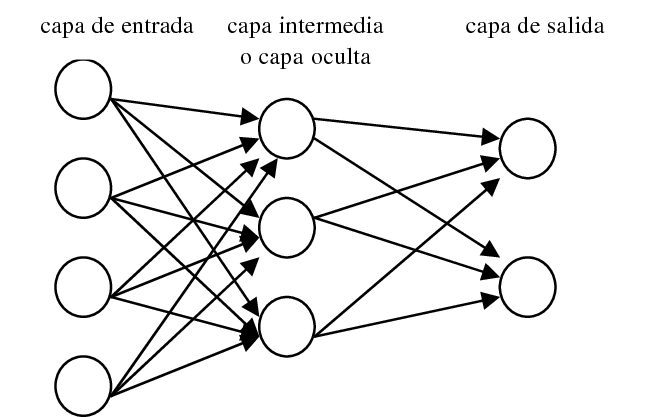
\includegraphics[scale=0.5]{2.png}
    \caption{Ejemplo visual de un árbol de decisión.}
    \label{fig:mesh1}
\end{figure}

\begin{figure}[h]
    \centering
    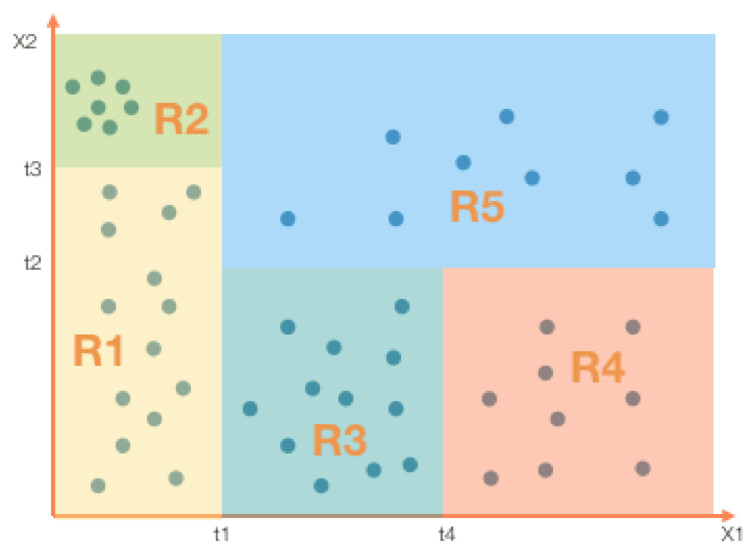
\includegraphics[scale=0.6]{3.jpg}
    \caption{Divisiones de los subconjuntos que realiza un árbol de decisión.}
    \label{fig:mesh1}
\end{figure}

\section{Resultados}
Para realizar la práctica se programó en lenguaje Python (revisar Anexo A) los dos sistemas de regresión. Primero se obtuvo el conjunto de datos publico mpg-auto el cual contiene información de distintos autos que se relacionan con el rendimiento de gasolina como se muestra en la Tabla 1. Para ambos casos se tuvo que hacer un pre-procesamiento de los datos debido a que el archivo disponible no cuenta con información completa para todos los registros. Es importante mencionar que el conjunto de datos contiene registros sobre el modelo y al ser una variable categorica puede ser convertida a variable dummy. Las variables se normalizaron para quedar en el mismo rango. los datos se dividieron para entrenamiento y pruebas en una proporcion 80/20 respectivamente.

Mediante la técnica de eliminación hacia atras se optimizó la regresión lineal multiple, colocando todas las variables x se fueron eliminando las variables que su valor P superaba el umbral del 5\% para el sistema.  En este conjunto de datos en particular solo se eliminó una variable la aceleración que si bien superaba el 5\% de umbral, no lo superó por mucho pues obtuvo 6\% y se pudo dejar en el modelo.  

\begin{table}[h]
\begin{center}
\begin{tabular}{| c | c |}
\hline
\multicolumn{2}{ |c| }{MPG-auto dataset} \\ \hline
Dato & Tipo de dato \\ \hline
Millas por galón & continuo \\ \hline
Cilindros & discreto multivalor \\ \hline
Desplazamiento & continuo \\ \hline
Caballos de fuerza & continua  \\ \hline
Peso & continuo  \\ \hline
Aceleración & continua   \\ \hline
Año del modelo &  discreto multivaluado  \\ \hline
Origen &  discreto multivaluado \\ \hline
Nombre del coche & cadena  \\ \hline
\end{tabular}
\caption{conjunto de datos MPG-auto }
\end{center}
\end{table}

Para los bosques aleatorios el proceso es similar, se ejecuta con el pre-procesamiento antes mencionado. Los resultados obtenidos se midieron mediante las metricas $R^2$ y $R^2$ ajustada como se observa en la Tabla 2.

\begin{table}[h]
\begin{center}
\begin{tabular}{| c | c |}
\hline
Regresión lineal multiple & Bosques aleatorios \\ \hline
$R^2$ = 82.54\% & $R^2$ = 82.27\% \\ \hline
$R^2$ = 82.54\% & $R^2$ = 88.22\% \\ \hline
\end{tabular}
\caption{Resultados del entrenamiento}
\end{center}
\end{table}

\section*{Conclusiones}
Como se pudo observar en los resultados, los bosques aleatorios son más robustos que la regresión lineal multiple aunque requiere más tiempo de procesamiento. Sin embargo, actualmente el poder de computo es cada vez mayor por lo que el tiempo se reduce con el paso de los años mediante el hardware. Durante el entrenamiento no se tomó en cuenta la variable categorica del modelo del auto ya que al intentar convertirla en variable dummy, eran demasiadas variables que no podian ser procesadas. Para trabajo futuro se puede modificar manualmente el conjunto de datos para asegurarse en reducir esa variable y colocar solo la marca del vehiculo. No se realizó en este trabajo ya que el rendimiento obtenido es considerablemente optimo por lo que podría no valer la pena incluir esas variables dummies. 

Las regresiones no son 100\% efectivas ya que no siempre se va a ajustar perfectamente a los valores a predecir pero si se puede hacer una aproximación cercana mediante la optimización de parametros de los métodos. Ademas, es bueno revisar de ser posible los datos que se proporcionan para el entrenamiento y eliminar los valores atipicos para evitar errores. El sobreajuste es un problema que trata de evitar los bosques aleatorios y que generalmente cumple su función, pero dependiendo de la aplicación puede optarse por una técnica u otra. A pesar de no ser confiables en su totalidad. las predicciones que es capaz de realizar alguno de estos métodos son lo suficientemente robustos para utilizarse en la industria ajustando el modelo lomejor posible para mejores resultados. 


\begin{thebibliography}{00}
\bibitem{b1}Yang, Q. (2017). Regression. In: Schintler, L., McNeely, C. (eds) Encyclopedia of Big Data. Springer, Cham. https://doi.org/10.1007/978-3-319-32001-4-174-1.
\bibitem{b2} Probabilidad y estadística aplicadas a la ingeniería, Douglas C. Montgomery y George C. Runger. Limusa Wiley, 2002. Segunda edición.
\bibitem{b3} Rokach, L., Maimon, O. (2005). Decision Trees. In: Maimon, O., Rokach, L. (eds) Data Mining and Knowledge Discovery Handbook. Springer, Boston, MA. https://doi.org/10.1007/0-387-25465-X-9.
\bibitem{b4} Cutler, A., Cutler, D.R., Stevens, J.R. (2012). Random Forests. In: Zhang, C., Ma, Y. (eds) Ensemble Machine Learning. Springer, Boston, MA. https://doi.org/10.1007/978-1-4419-9326-7-5.

\end{thebibliography}

\section{Anexo A}
Lectura de conjunto de datos y separandolos en variables dependientes e independientes y eliminación de valores incompletos.  
\lstset{language=Python, breaklines=true, basicstyle=\footnotesize}
\lstset{numbers=left, numberstyle=\tiny, stepnumber=1, numbersep=-2pt}
\begin{lstlisting}[frame=single]
    cols=["MPG", "cylinders", "displacement", "horsepower", "weight", "acceleration", "model year", "origin"]
    dataset=pd.read_csv("auto-mpg.data", na_values="?", comment='\t', sep=' ', skipinitialspace=True, names=cols)
    X=dataset.iloc[:,1:].values
    Y=dataset.iloc[:,0].values
\end{lstlisting}

Normalizado de datos. 
\begin{lstlisting}[frame=single]
    sc=StandardScaler()
    X=sc.fit_transform(X)
\end{lstlisting}

Separando el conjunto de datos.
\begin{lstlisting}[frame=single]
    X_train, X_test, Y_train, Y_test=train_test_split(X,Y,test_size=0.2, random_state=0)
\end{lstlisting}

\subsection{Regresión lineal multiple}

Ejecución de la regresión lineal multiple y calculo de las metricas de evaluación. 
\begin{lstlisting}[frame=single]
    regresion=LinearRegression()
    regresion.fit(X_train, Y_train)
    ypred=regresion.predict(X_test)

    print("R^2 : ", r2_score(Y_test, ypred))
    print("R^2 ajustada: ", 1 - (1-r2_score(Y_test, ypred))*(len(Y)-1)/(len(Y)-X.shape[1]-1))
\end{lstlisting}

\subsection{Bosques aleatorios}
Ejecución del bosque aleatorio estableciendo 10 árboles y calculo de las metricas de evaluación. 
\begin{lstlisting}[frame=single]
    regresion=RandomForestRegressor(n_estimators=10 ,random_state=0) 
    regresion.fit(X_train, Y_train)
    ypred=regresion.predict(X_test)
    
    print("R^2 : ", r2_score(Y_test, ypred))
    print("R^2 ajustada: ", 1 - (1-r2_score(Y_test, ypred))*(len(Y)-1)/(len(Y)-X.shape[1]-1))

\end{lstlisting}
\end{document}